
\documentclass[10pt]{article}
\usepackage{geometry} % see geometry.pdf on how to lay out the page. There's lots.
\geometry{a4paper} % or letter or a5paper or ... etc
% \geometry{landscape} % rotated page geometry
\usepackage[danish]{babel}
% See the ``Article customise'' template for come common customisations
\usepackage{fontspec}
\setmainfont[Ligatures=TeX]{Arial}
\usepackage[applemac]{inputenc}
\usepackage{graphicx}
\usepackage[colorlinks]{hyperref}
\title{Den videnskabelige poster}
\author{Thomas Mellergaard Amby}
\date{- 2015 -} % delete this line to display the current date

\parindent 0pt
%%% BEGIN DOCUMENT
\begin{document}

\maketitle
\tableofcontents
\clearpage 

\section{Introduktion:}
I den n�ste periode skal I som resultat af jeres anstrengelser i laboratoriet fremstille plakater, kaldet ``videnskabelig poster'' eller blot ``poster''. Det er en moderne m�de at formidle forskningsresultater. Det er \emph{sv�rt} at mestre denne pr�sentations form. Herunder ses et eksempel p� en poster.
\begin{figure}[h!]
	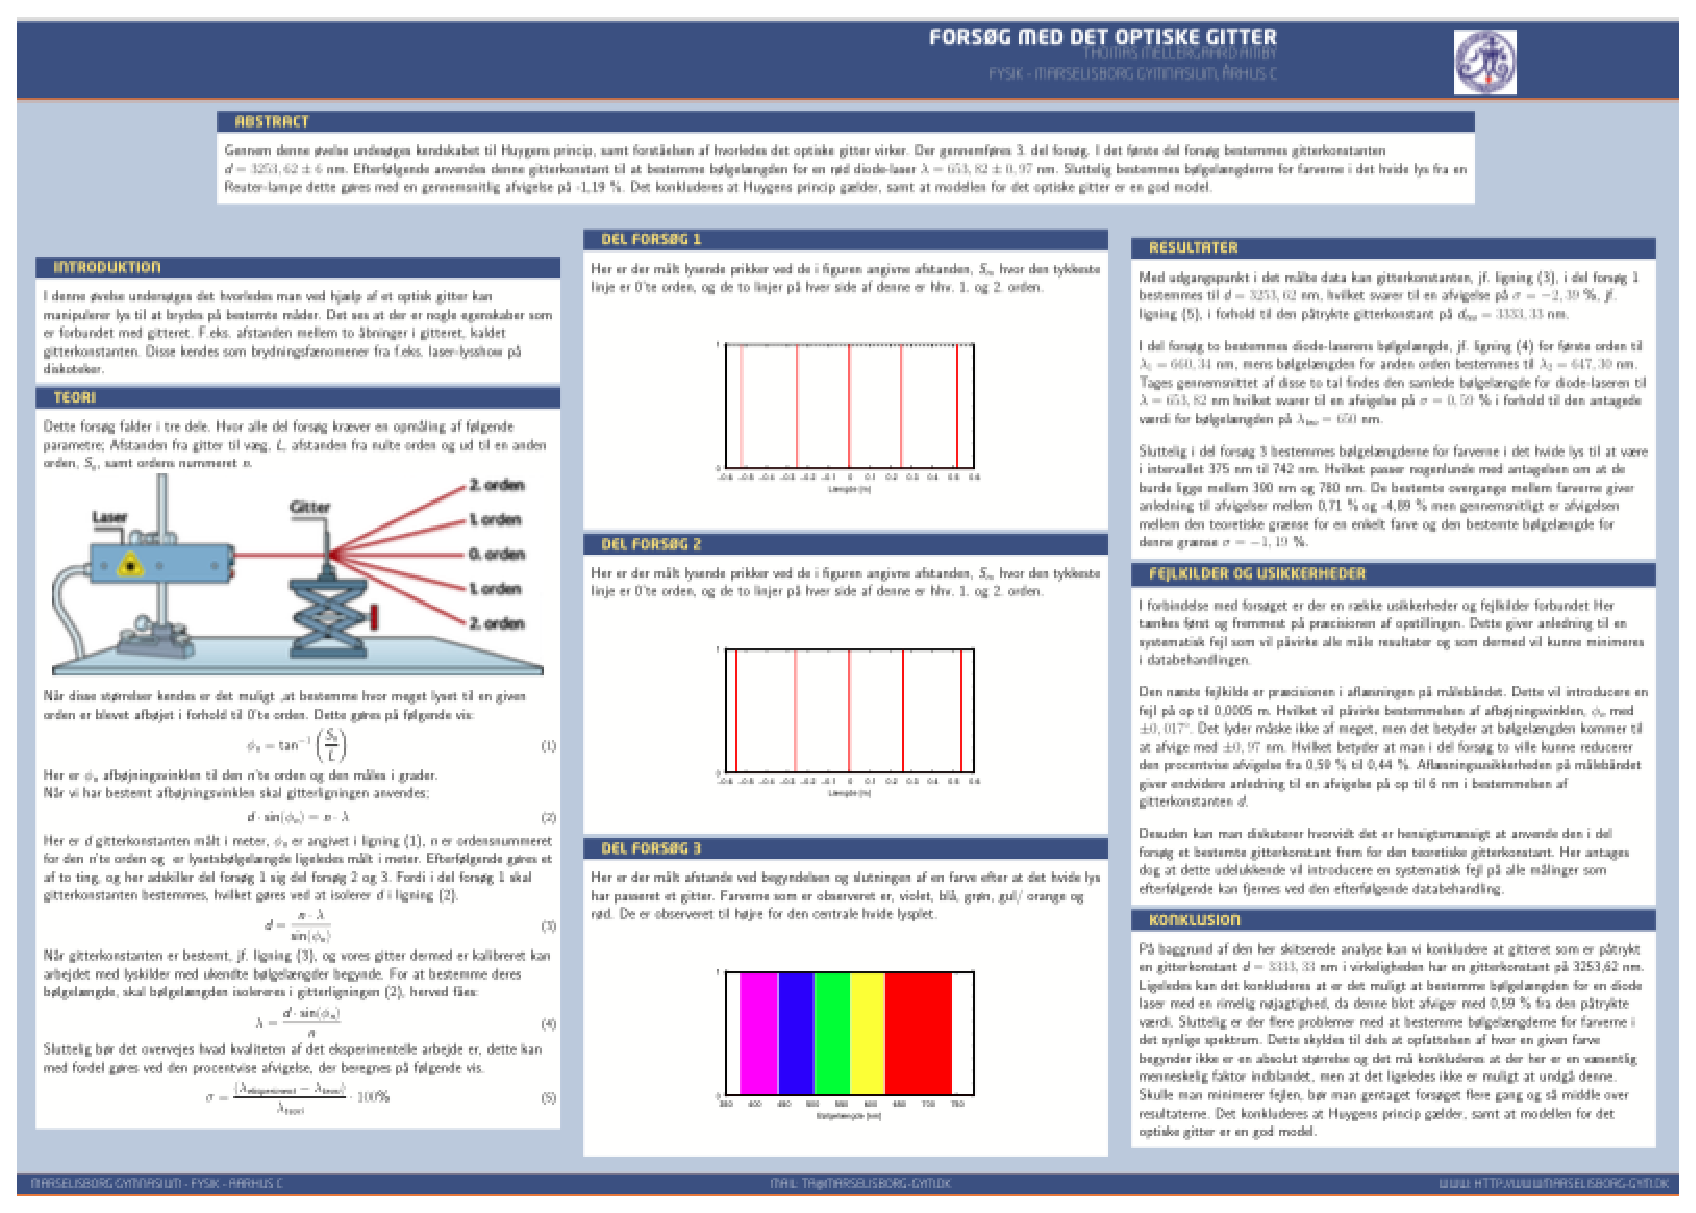
\includegraphics[width=\textwidth]{Pos-eks}
	\caption{Poster om fors�get det Optiske Gitter}
\end{figure}

\section{Formelle krav:}
Der er en r�kke krav til jeres poster, som I skal overholde. Posteren kan laves i PowerPoint eller et andet program efter jeres valg men der skal afleveres en pdf-fil.

Jeres poster skal:
\begin{itemize}
	\item v�re udf�rt i A1 format (I bestemmer om det skal v�re liggende eller st�ende).
	\item indeholde 2 - 3 figurer der understreger vigtige pointer p� posteren.
	\item gennemg� den teoretiske baggrund for fors�gene.
	\item indeholde et abstract, som kort gennemg�r form�let med �velsen, metoderne hvormed �velsen er gennemf�rt, resultaterne, usikkerheder/fejlkilder samt en konklusion.
\end{itemize}

\section{R�d og vejledninger:}
N�r man skal lave en poster skal man udf�rer alle de ting som man normalt skal n�r man laver en fysik rapport. Herefter skal rapporten koges ned. For en poster indeholder v�sentlig mindre tekst end rapporten. 

P� f�lgende hjemmesider finder I vink til hvordan man laver layoutet til en poster er I, i tvivl s� kom og sp�rg.
\begin{itemize}
	\item \href{http://colinpurrington.com/tips/academic/posterdesign}{http://colinpurrington.com/tips/academic/posterdesign}
	\item \href{http://hsp.berkeley.edu/sites/default/files/ScientificPosters.pdf}{http://hsp.berkeley.edu/sites/default/files/ScientificPosters.pdf}
	\item \href{http://www.makesigns.com/tutorials/}{http://www.makesigns.com/tutorials/}
\end{itemize}

Som program til at lave posteren foresl�r jeg at I anvender pr�sentations v�rkt�jer som f.eks. Power Point eller lignende.

\section{Disponering af elevtiden:}
N�r I har gennem�rt fors�get skal I anvende 2 timer pr. elev p� at fremstille en poster. Med alt det indhold som er n�dvendigt. Herefter f�r I et modul til at freml�gge jeres poster for en anden gruppe som giver jer konstruktiv feedback, og stille sp�rgsm�l til mig. De kommentarer som opponentgruppen kommer med, samt de svar jeg har givet p� evt. opklarende sp�rgsm�l, rettes nu i den resterende elevtid inden opgaven afleveres som anvist p� Lectio.

Herefter printer jeg posterne for jer og s� holder vi POSTER-session hvor posteren freml�gges mundtligt for mig, og resten af klassen.
\vfill
\begin{flushright}
God arbejdslyst\vspace{1cm}

Thomas
\end{flushright}

\end{document}